\subsubsection{UC27: Gestione delle categorie}
\label{sec:UC27}
\begin{figure}[!ht]
    \caption{Diagramma di UC27: Gestione delle categorie}
    \vspace{10px}
    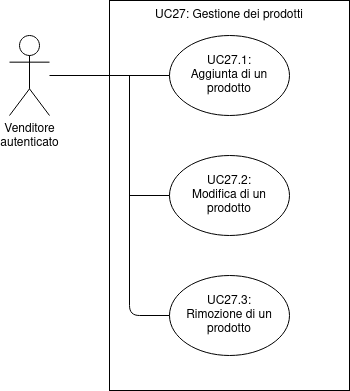
\includegraphics[scale=0.5]{../../../Images/AnalisiRequisiti/UC27}
    \centering
\end{figure}
\begin{itemize}
    \item \textbf{Descrizione:} sezione dove il venditore può gestire le categorie di prodotti del negozio;
    \item \textbf{Attore Primario:} venditore autenticato;
    \item \textbf{Precondizione:} il venditore si trova in una qualsiasi pagina della piattaforma;
    \item \textbf{Input:} il venditore clicca il bottone per entrare in questa sezione;
    \item \textbf{Postcondizione:} il venditore ha completato le operazioni sulle categorie;
    \item \textbf{Scenario Principale:}
          \begin{itemize}
              \item il venditore si trova nella pagina per la gestione del negozio;
              \item può decidere se aggiungere una nuova categoria o se rimuoverne una già presente;
              \item una volta terminato applica le modifiche.
          \end{itemize}
\end{itemize}
\subsubsubsection{UC27.1: Aggiunta di una categoria}
\label{sec:UC27.1}
\begin{itemize}
    \item \textbf{Descrizione:} sezione per aggiungere una categoria di prodotti nel negozio;
    \item \textbf{Attore Primario:} venditore autenticato;
    \item \textbf{Precondizione:} il venditore si trova nella sezione per gestire le categorie (\hyperref[sec:UC27]{\underline{UC27}});
    \item \textbf{Input:} il venditore inserisce tutti i dati relativi alla categoria da inserire;
    \item \textbf{Postcondizione:} la categoria è aggiunta e i clienti possono trovarla nel negozio;
    \item \textbf{Scenario Principale:}
          \begin{itemize}
              \item il venditore si trova nella sezione per gestire le categorie;
              \item il venditore decide di aggiungere una nuova categoria ed entra in questa sezione;
              \item inserisce tutti i dati richiesti;
              \item conferma l'aggiunta e la categoria è visibile nel negozio.
          \end{itemize}
\end{itemize}
\subsubsubsection{UC27.2: Rimozione di una categoria}
\label{sec:UC27.2}
\begin{itemize}
    \item \textbf{Descrizione:} sezione per rimuovere una categoria dal negozio;
    \item \textbf{Attore Primario:} venditore autenticato;
    \item \textbf{Precondizione:} il venditore si trova nella sezione per gestire le categorie (\hyperref[sec:UC27]{\underline{UC27}});
    \item \textbf{Input:} il venditore sceglie la categoria da rimuovere;
    \item \textbf{Postcondizione:} la categoria è stata rimossa dal negozio;
    \item \textbf{Scenario Principale:}
          \begin{itemize}
              \item il venditore si trova nella sezione per gestire le categorie;
              \item il venditore decide di rimuovere una categoria dal negozio;
              \item il venditore conferma la rimozione della categoria selezionata;
              \item la categoria non è più visibile nel negozio.
          \end{itemize}
\end{itemize}

